% ============================================================
% LIVRABLE 1 : RÉFÉRENTIEL DE DONNÉES
% Projet Cloud Healthcare Unit (CHU)
% Architecture Big Data pour le secteur de la santé
% ============================================================

\documentclass[12pt,a4paper]{article}

% ============================================================
% PACKAGES
% ============================================================
\usepackage[utf8]{inputenc}
\usepackage[T1]{fontenc}
\usepackage[french]{babel}
\usepackage[left=2.5cm,right=2.5cm,top=2.5cm,bottom=2.5cm]{geometry}
\usepackage{graphicx}
\usepackage{xcolor}
\usepackage{hyperref}
\usepackage{tabularx}
\usepackage{booktabs}
\usepackage{enumitem}
\usepackage{listings}
\usepackage{fancyhdr}
\usepackage{titlesec}
\usepackage{float}

% Fix fancyhdr header height warning
\setlength{\headheight}{15pt}
\usepackage{tikz}
\usepackage{amsmath}
\usepackage{amssymb}

% Configuration des liens hypertexte
\hypersetup{
    colorlinks=true,
    linkcolor=blue,
    filecolor=magenta,      
    urlcolor=cyan,
    pdftitle={Livrable 1 - Référentiel de données CHU},
    pdfauthor={Équipe Projet CHU},
}

% Configuration des en-têtes et pieds de page
\pagestyle{fancy}
\fancyhf{}
\fancyhead[L]{\leftmark}
\fancyhead[R]{Livrable 1 - CHU}
\fancyfoot[C]{\thepage}

% Style des titres de sections
\titleformat{\section}
{\normalfont\Large\bfseries\color{blue!70!black}}
{\thesection}{1em}{}

\titleformat{\subsection}
{\normalfont\large\bfseries\color{blue!50!black}}
{\thesubsection}{1em}{}

% Configuration de listings pour le code
\lstset{
    basicstyle=\ttfamily\small,
    breaklines=true,
    frame=single,
    backgroundcolor=\color{gray!10}
}

% ============================================================
% PAGE DE TITRE
% ============================================================
\begin{document}

\begin{titlepage}
    \centering
    \vspace*{2cm}
    
    {\Huge\bfseries Projet Big Data Healthcare\par}
    \vspace{0.5cm}
    {\LARGE Cloud Healthcare Unit (CHU)\par}
    \vspace{2cm}
    
    {\Huge\bfseries LIVRABLE 1\par}
    \vspace{0.5cm}
    {\Large Référentiel de Données\par}
    \vspace{0.3cm}
    {\large Modèle conceptuel et architecture de l'entrepôt\par}
    \vspace{2cm}
    
    {\large\itshape Équipe Projet :\par}
    {\large Nejma MOUALHI | Brieuc OLIVIERI | Nicolas TAING\par}
    \vspace{1cm}
    
    {\large Formation : CESI FISA A4\par}
    {\large Année universitaire : 2025-2026\par}
    \vspace{1.5cm}
    
    {\large Date : 10/10/2025\par}
    \vfill
    
    % Logo si disponible
    % \includegraphics[width=0.3\textwidth]{logo_etablissement.png}
    
\end{titlepage}

% ============================================================
% TABLE DES MATIÈRES
% ============================================================
\tableofcontents
\newpage

% ============================================================
% SECTION 1 : INTRODUCTION (COMPLÈTE)
% ============================================================
\section{Introduction}

\subsection{Contexte du projet CHU}

Le groupe hospitalier \textbf{Cloud Healthcare Unit (CHU)} souhaite se doter d'un système décisionnel capable d'exploiter efficacement la grande quantité de données issues de ses systèmes médicaux et administratifs.

Ces données, générées quotidiennement par les soins, les consultations, les hospitalisations, la satisfaction des patients et les registres de décès, constituent une ressource stratégique pour l'amélioration des soins et la performance des établissements. Cependant, leur volume, leur hétérogénéité et leur caractère sensible rendent leur exploitation complexe. Les infrastructures relationnelles classiques ne suffisent plus à absorber, traiter et analyser ces flux massifs tout en garantissant la conformité réglementaire.

Dans ce contexte, le projet \textbf{CHU – Cloud Healthcare Unit} vise à concevoir une infrastructure Big Data évolutive, sécurisée et performante, capable d'intégrer, de transformer et d'exposer les données de santé dans un cadre analytique cohérent. Cette architecture servira de base à la mise en place d'un entrepôt de données (Data Warehouse) dédié à la décision médicale et stratégique.

\subsection{Objectif global du système décisionnel Big Data}

L'objectif global est de mettre en œuvre un écosystème décisionnel complet permettant :

\begin{itemize}[leftmargin=*]
    \item d'intégrer des sources multiples (base PostgreSQL, fichiers CSV historiques, exports FTP) ;
    \item de garantir la sécurité et la confidentialité des données conformément au RGPD et à la certification HDS ;
    \item de modéliser les données sous une forme décisionnelle (faits et dimensions) afin de permettre une analyse par axes : temps, diagnostic, professionnel, établissement, etc. ;
    \item d'assurer des performances d'accès optimales grâce à un stockage distribué et des transformations massivement parallèles (Hadoop / Hive / Spark) ;
    \item et enfin, de favoriser la visualisation et la restitution des indicateurs via des outils comme Power BI.
\end{itemize}

\subsection{Enjeux du secteur médical}

Le secteur de la santé est aujourd'hui confronté à quatre enjeux majeurs :

\paragraph{Le volume et la variété} les établissements de santé génèrent des données massives, hétérogènes, issues de multiples systèmes (soins, satisfaction, mortalité, administratif).

\paragraph{La confidentialité} les données de santé relèvent de la catégorie des données sensibles (article 9 du RGPD). Leur stockage et leur traitement nécessitent des mesures strictes de pseudonymisation, de traçabilité et d'hébergement certifié HDS.

\paragraph{La performance} les utilisateurs attendent un accès rapide à l'information pour la prise de décision. Cela suppose un système capable de gérer des requêtes complexes sur de grands volumes en temps quasi réel.

\paragraph{L'évolutivité et la gouvernance} les besoins analytiques changent avec le temps. L'architecture doit rester ouverte, extensible et bien documentée pour permettre de nouvelles analyses sans remise en cause du modèle existant.

\subsection{But du livrable}

Ce premier livrable a pour but de définir le référentiel de données du futur système décisionnel du CHU. Il s'agit de la phase de conception conceptuelle, centrée sur :

\begin{itemize}[leftmargin=*]
    \item la définition de l'architecture Big Data et du pipeline d'intégration (ETLT) adapté aux données médicales ;
    \item la modélisation conceptuelle des données sous forme de faits et dimensions alignés sur les besoins des utilisateurs ;
    \item et la description des flux d'alimentation nécessaires à la constitution du futur entrepôt.
\end{itemize}

Ce travail jette les bases du modèle physique et de la phase d'implémentation à venir dans le livrable 2, garantissant la continuité entre la conception et la réalisation du système décisionnel.

% ============================================================
% SECTION 2 : ARCHITECTURE
% ============================================================
\newpage
\section{L'architecture Big Data}

\subsection{Choix de l'approche : ETLT}

\subsubsection{Justification du modèle}

Le choix du pipeline \textbf{ETLT (Extract – Transform – Load – Transform)} s'impose dans le contexte d'un projet manipulant des \textbf{données médicales sensibles}.
Contrairement à un \textbf{ETL classique}, où toutes les transformations précèdent le chargement, ou à un \textbf{ELT} où les données sont chargées brutes dans le cluster avant tout traitement, le modèle \textbf{ETLT} introduit une première transformation de \textbf{conformité} avant le stockage.

Cette étape intermédiaire répond à deux impératifs :

\begin{enumerate}[leftmargin=*]
    \item \textbf{Conformité réglementaire (RGPD / HDS)} : les données de santé ne peuvent pas être stockées dans leur forme brute, même temporairement, dans un environnement partagé. Une première transformation (T$_{1}$) est donc réalisée avant le chargement dans HDFS pour pseudonymiser, minimiser et normaliser les données sensibles.
    
    \item \textbf{Performance et évolutivité} : la deuxième transformation (T$_{2}$) est réalisée directement dans le cluster Big Data, à grande échelle, pour préparer les données au modèle décisionnel. Ce découplage permet de séparer les traitements \textbf{sécuritaires} (avant le stockage) des traitements \textbf{analytiques} (après le stockage).
\end{enumerate}
L'ETLT permet donc de \textbf{garantir la conformité} sans sacrifier la \textbf{scalabilité}.
C'est une approche hybride, combinant la rigueur du monde décisionnel et la puissance du Big Data distribué.

\subsubsection{Description du flux ETLT}

Le pipeline se compose de quatre étapes principales :

\paragraph{E – Extract}

L'extraction regroupe les données provenant de plusieurs sources :

\begin{itemize}[leftmargin=*]
    \item \textbf{PostgreSQL} : données médico-administratives des patients et des consultations.
    \item \textbf{Fichiers CSV} : exports des établissements hospitaliers, enquêtes de satisfaction, hospitalisations et registre des décès.
\end{itemize}

Les outils recommandés sont \textbf{Apache Sqoop} (pour les bases relationnelles) et \textbf{Apache Flume} ou \textbf{NiFi} (pour les flux de fichiers CSV).
Les données extraites sont ensuite validées (intégrité, schéma, doublons) avant de passer à l'étape suivante.

\paragraph{T$_{1}$ -- Transform Conformité}

Cette première transformation intervient \textbf{avant le stockage dans HDFS}.
Elle est dédiée à la \textbf{sécurité et la conformité} :

\begin{itemize}[leftmargin=*]
    \item \textbf{Pseudonymisation} : application d'un hachage salé sur les identifiants patients et professionnels de santé ;
    \item \textbf{Minimisation} : suppression des champs inutiles à l'analyse (adresse, téléphone, numéro de sécurité sociale, email) ;
    \item \textbf{Normalisation} : uniformisation des formats de dates, codes et unités ;
    \item \textbf{Contrôles} : validation du type, contraintes, dictionnaires (sexe, région, spécialité, diagnostic).
\end{itemize}

Les données ainsi transformées sont considérées comme \textit{pseudonymisées}, donc stockables dans un environnement Big Data certifié.

\paragraph{L – Load}

Le chargement consiste à \textbf{insérer les données pseudonymisées dans le Data Lake (HDFS)}.
Elles sont déposées dans la \textbf{zone Bronze (Landing)} sous leur forme semi-brute, accompagnées de métadonnées de traçabilité (source, date, checksum, version).
Les fichiers sont stockés au format \textbf{Parquet} ou \textbf{ORC}, optimisés pour le stockage colonne et la compression.

Chaque ingestion est historisée pour permettre la reconstitution d'un état passé (audit trail).

\paragraph{T$_{2}$ -- Transform Métier}

Cette deuxième transformation est exécutée directement dans le \textbf{cluster Big Data} (via \textbf{Spark} ou \textbf{Hive}) et correspond à la phase de \textbf{préparation analytique} :

\begin{itemize}[leftmargin=*]
    \item Nettoyage et harmonisation (référentiels communs, codes régionaux, tables FINESS) ;
    \item Conformation des dimensions (patient, professionnel, diagnostic, établissement, temps, satisfaction) ;
    \item Agrégations et calculs des indicateurs dans les \textbf{tables de faits} ;
    \item Génération du \textbf{modèle décisionnel en constellation} stocké dans la \textbf{zone Gold} du Data Lake.
\end{itemize}

Ce jeu de données devient la base du futur \textbf{entrepôt de données (Data Warehouse)}, exploitable via HiveQL, Power BI ou Tableau.

\subsubsection{Respect du RGPD et de la certification HDS}

L'architecture garantit la conformité réglementaire selon deux axes :

\paragraph{Technique}
\begin{itemize}[leftmargin=*]
    \item Pseudonymisation avant stockage (aucune donnée directement identifiable dans HDFS) ;
    \item HDFS configuré avec chiffrement au repos et journalisation d'accès ;
    \item Contrôle d'accès granulaire via \textbf{Apache Ranger} et authentification Kerberos ;
    \item Hébergement sur une infrastructure \textbf{certifiée HDS}.
\end{itemize}

\paragraph{Organisationnel}
\begin{itemize}[leftmargin=*]
    \item Politique de minimisation : seules les données strictement nécessaires aux analyses sont conservées ;
    \item Gestion des droits d'accès par rôle (RBAC) : distinction Data Engineer / Data Scientist / Analyste ;
    \item Journalisation des traitements et conservation limitée selon la durée légale ;
    \item Documentation et traçabilité complète des flux (Airflow + logs centralisés).
\end{itemize}

\subsection{Description des couches de l'architecture}

\subsubsection{Sources de données}

\begin{table}[H]
\centering
\caption{Récapitulatif des sources de données}
\begin{tabularx}{\textwidth}{|l|X|c|c|}
\hline
\textbf{Source} & \textbf{Description} & \textbf{Format} & \textbf{Volume estimé} \\
\hline
PostgreSQL – Consultation & Données des consultations : date, diagnostic, professionnel, patient & Relationnel & $\sim$1M lignes \\
\hline
PostgreSQL – Patient & Informations patients (pseudonymisées) & Relationnel & $\sim$100K lignes \\
\hline
CSV – Établissements & Référentiel national des hôpitaux (FINESS) & CSV & 24 colonnes \\
\hline
CSV – Hospitalisations & Données d'hospitalisation (durée, service, diagnostic) & CSV & Variable \\
\hline
CSV – Décès & Registre national des décès & CSV & Variable \\
\hline
CSV – Satisfaction & Enquêtes de satisfaction (2014–2020) & CSV (27 fichiers) & Variable \\
\hline
\end{tabularx}
\end{table}

\subsubsection{Zone Bronze (Landing)}

La \textbf{zone Bronze} correspond au \textbf{niveau d'atterrissage des données pseudonymisées}.
Les fichiers y sont stockés tels quels, sans modification de structure, afin de garantir la \textbf{traçabilité} et la \textbf{reproductibilité} des traitements.
Chaque dataset comporte un fichier de métadonnées (JSON ou Avro) décrivant :

\begin{itemize}[leftmargin=*]
    \item la source d'origine ;
    \item le schéma de données ;
    \item la date et l'heure d'ingestion ;
    \item le hash de contrôle et l'identifiant de version.
\end{itemize}

Cette zone est considérée comme \textbf{non exploitable directement} par les analystes — elle sert de référence brute pour les traitements en Silver.

\subsubsection{Zone Silver (Integration)}

La \textbf{zone Silver} regroupe les données \textbf{nettoyées, harmonisées et jointes} à partir des différentes sources Bronze.
Les opérations typiques sont :

\begin{itemize}[leftmargin=*]
    \item correspondance entre les identifiants patients/professionnels ;
    \item enrichissement à l'aide des référentiels (FINESS, géographie, spécialités) ;
    \item détection et suppression des doublons ;
    \item validation des clés étrangères.
\end{itemize}

Cette zone fournit des tables prêtes à être modélisées sous forme de faits et dimensions. Elle constitue l'espace de travail privilégié des \textbf{Data Engineers}.

\subsubsection{Zone Gold (Data Warehouse)}

La \textbf{zone Gold} représente la partie \textbf{décisionnelle} du Data Lake.
Les données y sont organisées selon un \textbf{modèle en constellation} :

\begin{itemize}[leftmargin=*]
    \item \textbf{Tables de faits} : Consultation, Hospitalisation, Décès, Satisfaction ;
    \item \textbf{Dimensions communes} : Temps, Patient, Professionnel, Établissement, Diagnostic, etc.
\end{itemize}

Ces tables sont stockées au format \textbf{ORC} (optimisé pour le requêtage SQL via Hive) et indexées pour accélérer les analyses.
Cette zone alimente directement les outils de \textbf{Business Intelligence} comme Power BI ou Tableau.

\subsubsection{Outils préconisés}

\begin{table}[H]
\centering
\caption{Stack technologique préconisée}
\begin{tabularx}{\textwidth}{|l|X|X|}
\hline
\textbf{Couche} & \textbf{Outil} & \textbf{Rôle principal} \\
\hline
Extraction & Apache Sqoop & Import depuis PostgreSQL \\
\hline
Extraction & Apache Flume / NiFi & Ingestion des fichiers CSV \\
\hline
Transformation & Apache Spark & Exécution des jobs T$_{1}$ et T$_{2}$ \\
\hline
Stockage & HDFS & Data Lake distribué \\
\hline
Data Warehouse & Apache Hive & Requêtage SQL et stockage ORC \\
\hline
Orchestration & Apache Airflow / NiFi & Séquencement, logs et monitoring \\
\hline
Sécurité & Apache Ranger & Contrôle d'accès granulaire, RBAC \\
\hline
Visualisation & Power BI / Tableau & Tableaux de bord interactifs \\
\hline
\end{tabularx}
\end{table}

\subsection{Analyse des données sources}

\subsubsection{Validation des volumes}

L'analyse des données réelles confirme les estimations du projet :

\begin{table}[H]
\centering
\caption{Volumes réels des données sources}
\begin{tabularx}{\textwidth}{|l|c|X|}
\hline
\textbf{Source} & \textbf{Volume réel} & \textbf{Commentaire} \\
\hline
PostgreSQL – Patient & 100 000 lignes & Volume idéal pour tests et prototypage \\
\hline
PostgreSQL – Consultation & 1 027 157 lignes & Confirme le challenge Big Data (1M+) \\
\hline
PostgreSQL – Professionnel & 1 048 575 lignes & Base complète des professionnels \\
\hline
PostgreSQL – Diagnostic & 15 490 codes & Référentiel CIM-10 complet \\
\hline
CSV – Satisfaction & 27 fichiers & Période 2014-2020, structure évolutive \\
\hline
CSV – Décès & Volume important & Fichier national, plusieurs Mo \\
\hline
\end{tabularx}
\end{table}

Ces volumes justifient pleinement l'approche Big Data : avec plus d'un million de consultations et la nécessité de croiser plusieurs sources hétérogènes, les technologies distribuées (Hadoop/Spark) s'imposent pour garantir la scalabilité.

\subsubsection{Schéma UML des données PostgreSQL}

L'analyse de la base de données PostgreSQL révèle un modèle relationnel classique qu'il faudra transformer en modèle dimensionnel :

\begin{figure}[H]
\centering
\includegraphics[width=0.9\textwidth]{uml.png}
\caption{Schéma UML des tables PostgreSQL sources}
\label{fig:uml_postgresql}
\end{figure}

\subsubsection{Justification des choix architecturaux}

Cette analyse des données réelles confirme nos choix techniques :

\paragraph{Nécessité de la pseudonymisation}
Les tables contiennent des données hautement sensibles (nom, prénom, email, téléphone, numéro de sécurité sociale). La transformation T$_{1}$ doit impérativement les pseudonymiser avant stockage dans HDFS.

\paragraph{Complexité des jointures}
Le modèle relationnel impose de multiples jointures (Patient$\leftrightarrow$Consultation$\leftrightarrow$Professionnel$\leftrightarrow$Diagnostic). Le modèle dimensionnel en constellation simplifiera grandement les requêtes analytiques.

\paragraph{Hétérogénéité des formats}
PostgreSQL utilise des types \texttt{date} et \texttt{time} normalisés, mais les CSV utilisent des formats texte variés. La couche Silver d'intégration est cruciale pour harmoniser ces formats.

\paragraph{Volume justifiant le Big Data}
Avec 1M+ de consultations et la perspective de croissance, les jointures sur des tables relationnelles classiques deviendraient rapidement prohibitives. Le stockage colonnaire (ORC) et le parallélisme (Spark) sont nécessaires.

\subsection{Schéma global de l'architecture}

\begin{figure}[H]
\centering
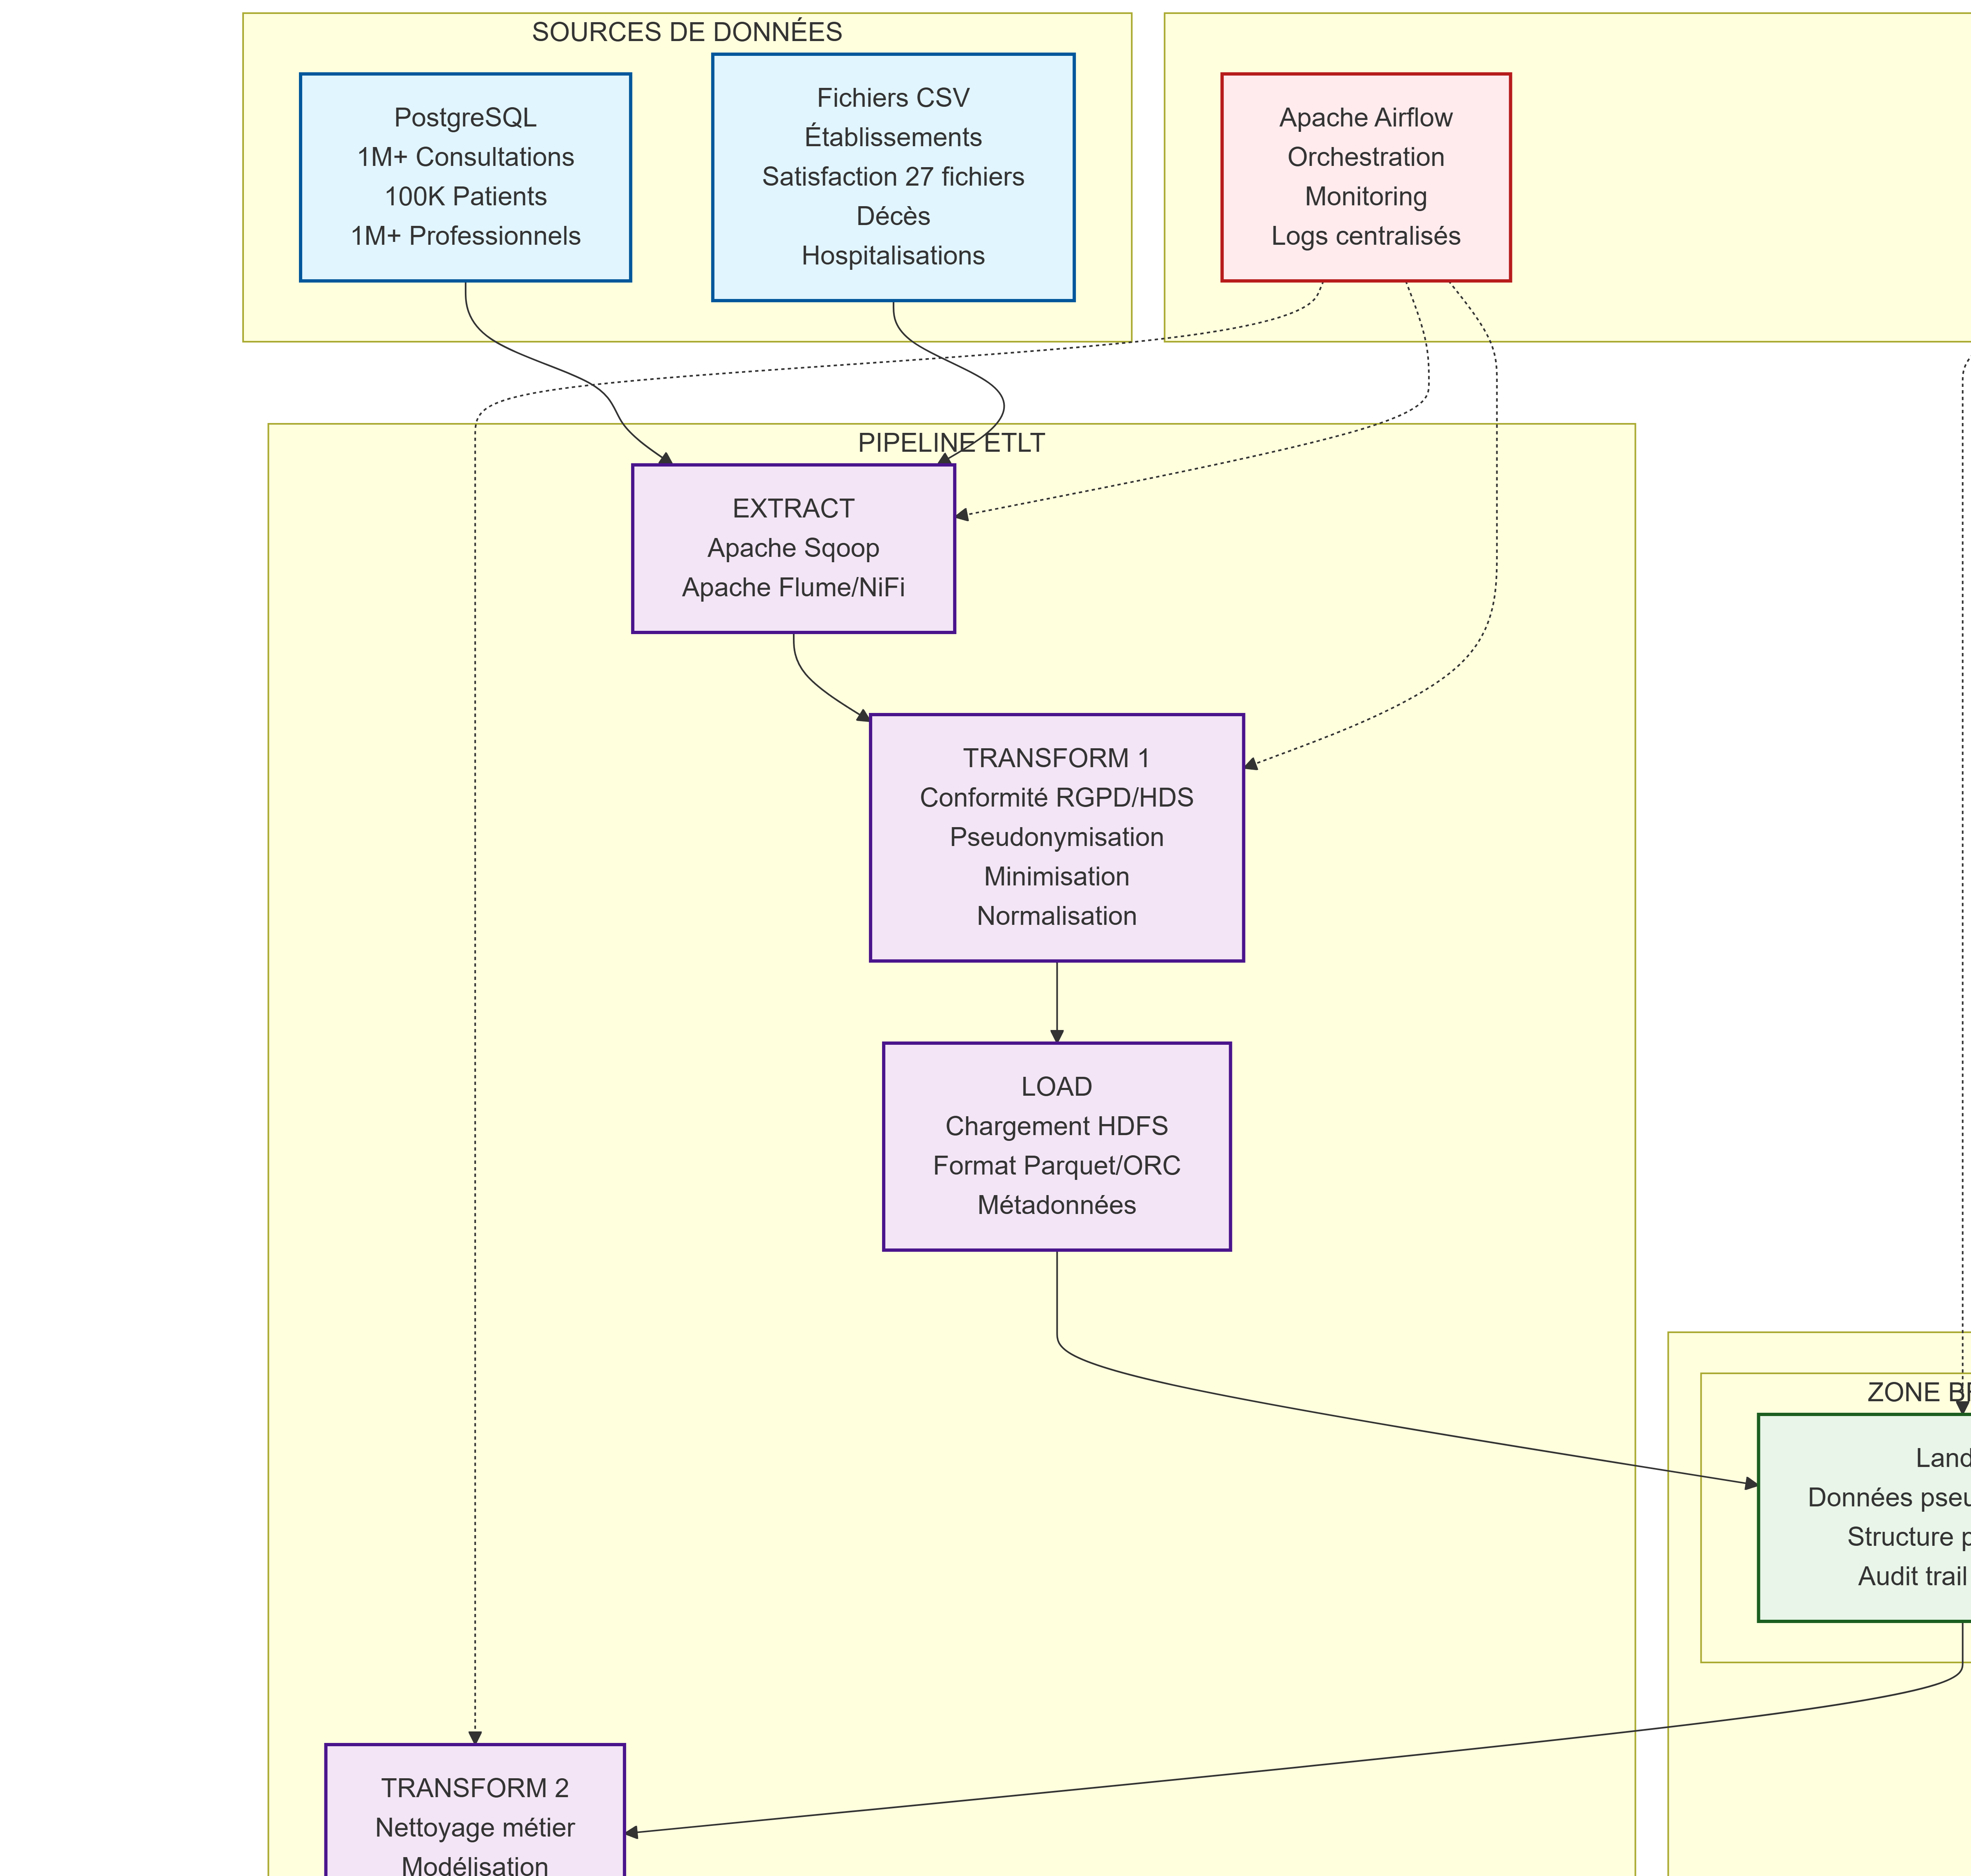
\includegraphics[width=\textwidth]{archi_etlt.png}
\caption{Architecture ETLT avec zones Bronze/Silver/Gold}
\label{fig:architecture_etlt}
\end{figure}



% ============================================================
% SECTION 3 : MODÈLE CONCEPTUEL (À DÉVELOPPER)
% ============================================================
\newpage
\section{Modèle conceptuel de données}

\subsection{Identification des axes d'analyse (dimensions)}

\subsubsection{Dimension Temps}

La dimension Temps constitue l’un des axes fondamentaux d’analyse décisionnelle. Elle permet de contextualiser l’ensemble des faits médicaux, administratifs et de satisfaction selon une perspective temporelle. L’analyse temporelle est essentielle pour évaluer l’évolution des taux d’hospitalisation, des consultations ou des décès et pour mettre en évidence des tendances saisonnières, des pics d’activité ou des améliorations des soins sur une période donnée.

Sources de données : horodatages présents dans les systèmes hospitaliers (dates d’admission, de consultation, de diagnostic, de décès, etc.) et fichiers plats / bases fournis par le groupe CHU.

Structure :
\begin{itemize}
    \item \texttt{id\_temps} (clé primaire)
    \item date\_complète
    \item jour, mois, année
    \item trimestre, semaine, jour\_semaine
    \item indicateurs saisonniers (jour férié, week-end, période estivale, etc.)
\end{itemize}

Usage analytique : permet de croiser les faits avec la temporalité pour mesurer des tendances (évolution mensuelle du taux d’hospitalisation, périodes de surcharge, évolution de la satisfaction, etc.).

\subsubsection{Dimension Patient}

La dimension Patient regroupe les informations démographiques et administratives des individus pris en charge par les établissements du groupe CHU. Elle permet une analyse fine de la population soignée selon des critères d’âge, de sexe et de profil socio-démographique.

Sources de données : principalement la base PostgreSQL médico-administrative, enrichie par des fichiers CSV des services d’état civil ou de suivi patient.

Structure :
\begin{itemize}
    \item \texttt{id\_patient} (clé primaire)
    \item sexe
    \item date\_naissance / âge
    \item catégorie d’âge
    \item situation géographique (région / département)
    \item statut de vie (vivant / décédé)
\end{itemize}

Usage analytique : taux d’hospitalisation par tranche d’âge, répartition des consultations par sexe, corrélation âge / satisfaction, segmentation patient.

\subsubsection{Dimension Professionnel de santé}

La dimension Professionnel décrit le personnel médical et paramédical impliqué dans les soins. Elle offre une vue sur la distribution et l’efficacité des équipes soignantes.

Sources de données : systèmes RH hospitaliers et bases de gestion des ressources humaines du groupe CHU.

Structure :
\begin{itemize}
    \item \texttt{id\_professionnel} (clé primaire)
    \item nom, prénom (pseudonymisés si nécessaire)
    \item spécialité médicale
    \item statut (médecin, infirmier, aide-soignant, etc.)
    \item service / établissement d’affectation
    \item ancienneté / charge de travail moyenne
\end{itemize}

Usage analytique : répartition des actes par professionnel, taux de consultation par spécialité, impact de l’expérience sur la satisfaction patient.

\subsubsection{Dimension Diagnostic}

La dimension Diagnostic regroupe les pathologies identifiées lors des consultations ou hospitalisations. Elle permet d’analyser la répartition et la fréquence des maladies, ainsi que leur lien avec les soins prodigués.

Sources de données : systèmes médicaux du CHU et codes diagnostics (CIM‑10 ou équivalents).

Structure :
\begin{itemize}
    \item \texttt{id\_diagnostic} (clé primaire)
    \item code\_diagnostic (CIM‑10)
    \item libelle\_diagnostic
    \item catégorie\_pathologie
    \item gravité / type d’intervention associée
\end{itemize}

Usage analytique : prévalence des pathologies, taux d’hospitalisation par diagnostic, corrélations diagnostic / durée moyenne de séjour.

\subsubsection{Dimension Établissement}

La dimension Établissement décrit les structures de santé (hôpitaux, cliniques, établissements publics ou privés) rattachées au groupe CHU. Elle est essentielle pour la comparaison inter-établissements et le suivi de la performance hospitalière.

Sources de données : fichier CSV national des établissements (FINESS) et systèmes d’information internes du CHU.

Structure :
\begin{itemize}
    \item \texttt{id\_etablissement} (clé primaire)
    \item nom\_etablissement
    \item type\_etablissement (CHU, clinique, centre régional, etc.)
    \item capacité d’accueil (nombre de lits)
    \item région / département
    \item code\_Finess
    \item spécialité principale
\end{itemize}

Usage analytique : comparaison de fréquentation, identification des zones les plus sollicitées, suivi de la performance opérationnelle par taille ou spécialité.

\subsubsection{Dimension Localisation}

La dimension Localisation fournit la perspective géographique des analyses. Elle relie les faits aux zones administratives et sanitaires (régions, départements, communes).

Sources de données : fichiers d’état civil, base nationale des établissements hospitaliers, coordonnées géographiques des établissements et des patients.

Structure :
\begin{itemize}
    \item \texttt{id\_localisation} (clé primaire)
    \item région, département, commune
    \item code\_postal
    \item zone\_urbaine / rurale
    \item coordonnées GPS
\end{itemize}

Usage analytique : cartographie de la répartition des patients, mortalité ou satisfaction par région, détection de zones sous-dotées en infrastructures.

\subsubsection{Dimension Satisfaction}

La dimension Satisfaction évalue la perception des patients sur la qualité des soins reçus. Elle est essentielle pour le pilotage de la qualité hospitalière et l’amélioration continue.

Sources de données : fichiers plats de satisfaction patient et enquêtes administrées par les établissements du CHU.

Structure :
\begin{itemize}
    \item \texttt{id\_satisfaction} (clé primaire)
    \item note\_globale
    \item critères (accueil, propreté, qualité du soin, disponibilité du personnel)
    \item année / période d’enquête
    \item source de collecte (en ligne, papier, entretien)
\end{itemize}

Usage analytique : indicateurs de satisfaction par établissement ou région, suivi temporel du ressenti patient, corrélation satisfaction / performance médicale.

\subsection{Identification des faits et mesures}

\subsubsection{Fait Consultation}

La table \textbf{FAIT\_CONSULTATION} centralise les informations relatives aux consultations médicales réalisées dans les établissements du groupe CHU. Elle permet d’analyser l’activité des praticiens, la fréquentation des patients et les tendances de consultation selon différents axes (temps, localisation, diagnostic, professionnel, etc.). Cette table constitue un indicateur opérationnel clé traduisant la demande de soins au sein du réseau hospitalier.

Objectifs analytiques :
\begin{itemize}
    \item mesurer le taux de consultation par période, région ou diagnostic ;
    \item suivre la distribution des consultations selon le sexe, l’âge et le profil socio-démographique ;
    \item évaluer la charge d’activité des professionnels ;
    \item identifier les évolutions de la demande de soins dans le temps.
\end{itemize}

Liens dimensionnels :
\begin{itemize}
    \item \texttt{DIM\_TEMPS} : date de la consultation ;
    \item \texttt{DIM\_PATIENT} : informations démographiques du patient ;
    \item \texttt{DIM\_PROFESSIONNEL} : praticien effectuant la consultation ;
    \item \texttt{DIM\_ETABLISSEMENT} : lieu de la consultation ;
    \item \texttt{DIM\_DIAGNOSTIC} : motif ou résultat de la consultation ;
    \item \texttt{DIM\_LOCALISATION} : région / département associés.
\end{itemize}

Granularité : une ligne = une consultation (horodatage précis, patient, professionnel, diagnostic).

Mesures principales :
\begin{itemize}
    \item \texttt{nb\_consultations} : nombre de consultations ;
    \item \texttt{duree\_consultation\_moyenne} : durée moyenne par consultation ;
    \item \texttt{taux\_consultation\_par\_diagnostic} ;
    \item \texttt{taux\_consultation\_par\_professionnel} .
\end{itemize}

\subsubsection{Fait Hospitalisation}

La table \textbf{FAIT\_HOSPITALISATION} regroupe les données relatives aux séjours hospitaliers. Elle est destinée aux analyses d’occupation, de durée de séjour et de répartition des pathologies hospitalisées, et sert de référence pour le pilotage des capacités et de la performance clinique.

Objectifs analytiques :
\begin{itemize}
    \item mesurer le taux d’hospitalisation par période, région et diagnostic ;
    \item calculer la durée moyenne de séjour (DMS) par pathologie et profil patient ;
    \item analyser la fréquence d’hospitalisation par sexe et tranche d’âge ;
    \item estimer le taux d’occupation des lits et services hospitaliers.
\end{itemize}

Liens dimensionnels :
\begin{itemize}
    \item \texttt{DIM\_TEMPS} : date d’entrée, date de sortie ;
    \item \texttt{DIM\_PATIENT} : profil du patient hospitalisé ;
    \item \texttt{DIM\_DIAGNOSTIC} : motif d’hospitalisation ;
    \item \texttt{DIM\_ETABLISSEMENT} : établissement d’accueil ;
    \item \texttt{DIM\_PROFESSIONNEL} : médecin référent ;
    \item \texttt{DIM\_LOCALISATION} : position géographique de l’établissement.
\end{itemize}

Granularité : une ligne = un séjour hospitalier (entrant, sortant, diagnostics associés).

Mesures principales :
\begin{itemize}
    \item \texttt{nb\_hospitalisations} ;
    \item \texttt{duree\_sejour\_moyenne} (jours) ;
    \item \texttt{taux\_occupation} (lits occupés / lits disponibles) ;
    \item \texttt{taux\_hospitalisation\_par\_diagnostic}.
\end{itemize}

\subsubsection{Fait Satisfaction}

La table \textbf{FAIT\_SATISFACTION} consolide les résultats des enquêtes de satisfaction patient menées après une consultation ou un séjour. Elle sert à piloter la qualité perçue et à orienter les actions d’amélioration.

Objectifs analytiques :
\begin{itemize}
    \item calculer le taux de satisfaction global par établissement, région et période ;
    \item analyser les critères de satisfaction (accueil, propreté, qualité du soin, disponibilité du personnel) ;
    \item suivre l’évolution temporelle des indicateurs de satisfaction ;
    \item corréler satisfaction, durée de séjour et typologie de pathologie.
\end{itemize}

Liens dimensionnels :
\begin{itemize}
    \item \texttt{DIM\_TEMPS} : période / date d’enquête ;
    \item \texttt{DIM\_PATIENT} : répondant (anonymisé) ;
    \item \texttt{DIM\_ETABLISSEMENT} : établissement concerné ;
    \item \texttt{DIM\_SATISFACTION} : codification des critères ;
    \item \texttt{DIM\_LOCALISATION} : zone géographique du répondant.
\end{itemize}

Granularité : une ligne = une réponse d’enquête (ou agrégation par sondage selon disponibilité).

Mesures principales :
\begin{itemize}
    \item \texttt{note\_satisfaction\_moyenne} ;
    \item \texttt{taux\_reclamation} ;
    \item \texttt{indice\_qualite\_service} ;
    \item \texttt{nb\_enquetes\_realisees}.
\end{itemize}

\subsubsection{Fait Décès}

La table \textbf{FAIT\_DECES} centralise les informations issues des registres de décès et permet d’analyser la mortalité selon des critères temporels, géographiques et médicaux. Elle alimente les analyses épidémiologiques et de planification sanitaire.

Objectifs analytiques :
\begin{itemize}
    \item étudier la répartition des décès par région et période ;
    \item identifier les diagnostics associés aux décès ;
    \item mesurer le taux de mortalité hospitalière ;
    \item croiser les décès avec les caractéristiques patient (âge, sexe, établissement).
\end{itemize}

Liens dimensionnels :
\begin{itemize}
    \item \texttt{DIM\_TEMPS} : date du décès ;
    \item \texttt{DIM\_PATIENT} : caractéristiques du défunt ;
    \item \texttt{DIM\_ETABLISSEMENT} : lieu du décès (si hospitalier) ;
    \item \texttt{DIM\_DIAGNOSTIC} : cause principale du décès ;
    \item \texttt{DIM\_LOCALISATION} : région / commune de décès.
\end{itemize}

Granularité : une ligne = un acte de décès déclaré (avec diagnostics codés si disponibles).

Mesures principales :
\begin{itemize}
    \item \texttt{nb\_deces} ;
    \item \texttt{taux\_mortalite} (décès / population hospitalisée) ;
    \item \texttt{age\_moyen\_deces} ;
    \item \texttt{taux\_deces\_par\_diagnostic}.
\end{itemize}

\subsection{Modélisation conceptuelle (diagramme constellation)}

\subsubsection{Présentation graphique}

Le modèle dimensionnel adopte une architecture en constellation avec 4 tables de faits interconnectées par 8 dimensions. Ce schéma permet d'analyser l'activité hospitalière selon différents processus métier tout en partageant des dimensions communes (Temps, Patient, Établissement, Diagnostic).

\begin{figure}[H]
\centering
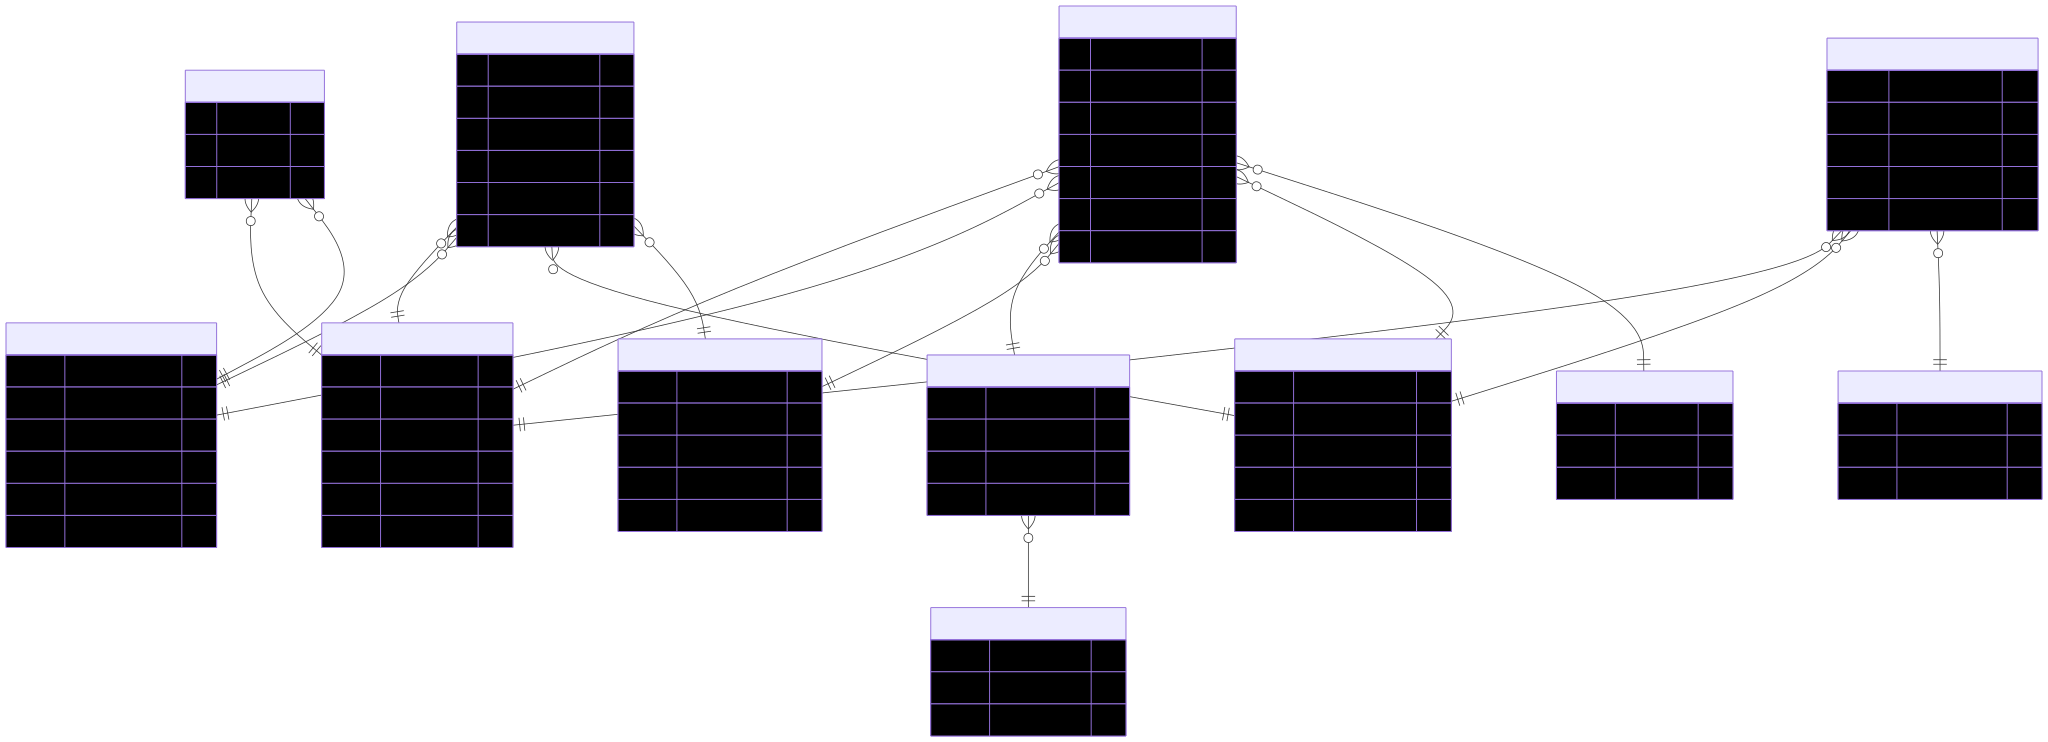
\includegraphics[width=\textwidth]{diagramme_dimensions.svg}
\caption{Schéma en constellation du modèle dimensionnel CHU}
\label{fig:constellation}
\end{figure}

Le diagramme illustre les relations entre les 4 tables de faits (Consultation, Hospitalisation, Décès, Satisfaction) et les 8 dimensions identifiées. Les dimensions communes (en bleu) sont partagées entre plusieurs faits, tandis que les dimensions spécifiques (en vert) ne concernent qu'un seul processus métier.

\subsubsection{Justification du modèle constellation}

Le choix d'une architecture en constellation repose sur l'analyse des processus métier distincts du groupe CHU :

\paragraph{Quatre processus métier indépendants}
\begin{itemize}[leftmargin=*]
    \item \textbf{Consultation} : activité ambulatoire des professionnels de santé
    \item \textbf{Hospitalisation} : séjours avec durée et gestion des lits
    \item \textbf{Décès} : mortalité avec contexte géographique
    \item \textbf{Satisfaction} : enquêtes de qualité perçue
\end{itemize}

\paragraph{Dimensions communes partagées}
Les dimensions Temps, Patient, Établissement et Diagnostic sont réutilisées par plusieurs faits, ce qui garantit la cohérence des analyses croisées et réduit la redondance.

\paragraph{Dimensions spécifiques métier}
Certaines dimensions ne concernent qu'un seul processus : Professionnel et Mutuelle pour les consultations, Type\_Enquête pour la satisfaction. Cette spécialisation évite la pollution dimensionnelle et simplifie les modèles.

\paragraph{Avantages du modèle constellation}
\begin{itemize}[leftmargin=*]
    \item Séparation logique des processus métier distincts
    \item Réutilisation optimale des dimensions communes
    \item Flexibilité pour ajouter de nouveaux faits sans refonte globale
    \item Performance des requêtes par processus (pas de sur-dimensionnement)
\end{itemize}

\subsubsection{Relations clés entre faits et dimensions}

Le tableau suivant récapitule les dimensions liées à chaque table de faits :

\begin{table}[H]
\centering
\caption{Récapitulatif des relations faits-dimensions}
\begin{tabularx}{\textwidth}{|l|X|}
\hline
\textbf{Table de faits} & \textbf{Dimensions liées} \\
\hline
FAIT\_CONSULTATION & DIM\_TEMPS, DIM\_PATIENT, DIM\_PROFESSIONNEL, DIM\_DIAGNOSTIC, DIM\_ETABLISSEMENT, DIM\_MUTUELLE \\
\hline
FAIT\_HOSPITALISATION & DIM\_TEMPS (entrée + sortie), DIM\_PATIENT, DIM\_ETABLISSEMENT, DIM\_DIAGNOSTIC \\
\hline
FAIT\_DECES & DIM\_TEMPS, DIM\_PATIENT \\
\hline
FAIT\_SATISFACTION & DIM\_TEMPS, DIM\_ETABLISSEMENT, DIM\_TYPE\_ENQUETE \\
\hline
\end{tabularx}
\end{table}

Cette structure en constellation permet d'analyser chaque processus métier de manière autonome tout en conservant la cohérence globale grâce aux dimensions partagées.

% ============================================================
% SECTION 4 : JOBS D'ALIMENTATION (À DÉVELOPPER)
% ============================================================
\newpage
\section{Jobs d'alimentation (vue conceptuelle)}

\subsection{Objectifs}

Cette section présente la conception globale des jobs d'alimentation destinés à automatiser la préparation et le chargement des données dans le futur entrepôt décisionnel. L'objectif est de définir une vision fonctionnelle et séquentielle du traitement des données, avant la phase de développement qui sera réalisée avec Talend Open Studio dans le livrable suivant.

Les principaux objectifs sont :

\begin{itemize}[leftmargin=*]
    \item Garantir la qualité et la traçabilité des flux de données tout au long du processus
    \item Assurer la conformité RGPD/HDS dès les premières étapes d'ingestion
    \item Préparer le futur entrepôt décisionnel et les tables de faits/dimensions nécessaires à la restitution
    \item Structurer une chaîne d'alimentation claire et rejouable en cas d'erreur ou d'évolution des sources
    \item Favoriser la standardisation des étapes pour faciliter l'industrialisation future dans Talend
\end{itemize}

\subsection{Description des jobs}

La table suivante illustre les principaux jobs d'alimentation prévus dans le cadre du projet. Ils sont organisés en deux grandes phases :

\begin{itemize}[leftmargin=*]
    \item \textbf{T$_{1}$} : Préparation et nettoyage des données sources (qualité, pseudonymisation, normalisation)
    \item \textbf{T$_{2}$} : Construction du modèle décisionnel (dimensions, faits, indicateurs)
\end{itemize}

Il s'agit ici d'une vue conceptuelle et non technique ; les noms et étapes sont susceptibles d'évoluer lors du développement avec Talend.

\begin{table}[H]
\centering
\caption{Liste des jobs d'alimentation}
\begin{tabularx}{\textwidth}{|l|c|X|}
\hline
\textbf{Job} & \textbf{Étape} & \textbf{Rôle principal} \\
\hline
J-T$_{1}$-Patient & T$_{1}$ & Pseudonymisation et suppression des informations personnelles (PII) pour conformité RGPD \\
\hline
J-T$_{1}$-Consultation & T$_{1}$ & Normalisation des dates, harmonisation des structures de fichiers et des schémas \\
\hline
J-T$_{1}$-Etablissement & T$_{1}$ & Nettoyage des adresses, validation des identifiants FINESS, contrôle des doublons \\
\hline
J-T$_{1}$-Deces & T$_{1}$ & Pseudonymisation et agrégation des données de mortalité par année et par région \\
\hline
J-T$_{1}$-Satisfaction & T$_{1}$ & Harmonisation des enquêtes de satisfaction (ESATIS48H, ESATISCA 2020) et formats multiples \\
\hline
\hline
J-Dim\_Temps & T$_{2}$ & Génération d'un calendrier décisionnel complet (jour, mois, trimestre, année) \\
\hline
J-Dim\_Patient & T$_{2}$ & Construction de la dimension patient à partir des données pseudonymisées \\
\hline
J-Dim\_Etablissement & T$_{2}$ & Mapping des établissements, rattachement régional et fusion des sources \\
\hline
J-Dim\_Diagnostic & T$_{2}$ & Structuration de la hiérarchie CIM-10 pour les diagnostics médicaux \\
\hline
J-Dim\_Professionnel & T$_{2}$ & Regroupement des professionnels de santé et jointure sur spécialité \\
\hline
J-Dim\_Specialite & T$_{2}$ & Intégration du référentiel des spécialités médicales \\
\hline
J-Dim\_Mutuelle & T$_{2}$ & Construction de la dimension mutuelle et adhésions patients \\
\hline
J-Dim\_Type\_Enquete & T$_{2}$ & Création de la typologie des enquêtes de satisfaction \\
\hline
\hline
J-Fait\_Consultation & T$_{2}$ & Agrégation des consultations selon les axes d'analyse (année, région, diagnostic) \\
\hline
J-Fait\_Hospitalisation & T$_{2}$ & Calcul des durées moyennes de séjour et indicateurs par établissement \\
\hline
J-Fait\_Deces & T$_{2}$ & Croisement localisation / temps pour suivi de la mortalité \\
\hline
J-Fait\_Satisfaction & T$_{2}$ & Pivot et agrégation des indicateurs de satisfaction par établissement et région \\
\hline
\end{tabularx}
\end{table}

\subsection{Séquencement et dépendances}

L'exécution des jobs suivra une logique séquentielle structurée en deux phases :

\paragraph{Phase T$_{1}$ -- Préparation des données}
Ingestion, contrôle de conformité et harmonisation des fichiers sources. Les jobs de cette phase garantissent la qualité et la cohérence des données avant toute intégration. Les jobs T$_{1}$ sont indépendants et peuvent s'exécuter en parallèle.

\paragraph{Phase T$_{2}$ -- Construction du modèle décisionnel}
Création des dimensions (temps, établissement, patient) et des faits (hospitalisations, satisfaction). Ces jobs permettent d'alimenter la base décisionnelle qui servira ensuite à la production d'indicateurs pour Power BI.

Dépendances principales :
\begin{itemize}[leftmargin=*]
    \item Les jobs T$_{2}$ dépendent de la complétion de tous les jobs T$_{1}$ correspondants
    \item Les jobs de construction des dimensions doivent précéder les jobs de construction des faits
    \item Les jobs de faits peuvent s'exécuter en parallèle une fois toutes les dimensions créées
\end{itemize}

Un diagramme de séquence ou DAG (Airflow ou Talend) sera développé dans le Livrable 2, afin de visualiser les dépendances entre jobs, leurs ordres d'exécution, et les points de contrôle de qualité.

\subsection{Perspective : implémentation sous Talend (Livrable 2)}

La prochaine étape du projet consistera à développer ces jobs dans Talend Open Studio, en transformant la conception présentée ici en chaîne d'intégration automatisée. Chaque job sera matérialisé sous forme de flux Talend intégrant :

\begin{itemize}[leftmargin=*]
    \item des composants de lecture et transformation des données sources
    \item des contrôles de qualité (cohérence, complétude, unicité)
    \item des liens logiques entre les tables de faits et de dimensions
    \item une publication automatisée des jeux validés vers le schéma décisionnel
\end{itemize}

Cette mise en œuvre permettra de passer d'une architecture théorique à un flux décisionnel complet et opérationnel, garantissant la fiabilité et la reproductibilité des chargements de données.

% ============================================================
% SECTION 5 : CONCLUSION
% ============================================================
\newpage
\section{Conclusion et prochaines étapes}

\subsection{Synthèse du livrable}

Ce premier livrable a permis de définir le référentiel de données du système décisionnel CHU. Les principaux livrables sont :

\begin{itemize}[leftmargin=*]
    \item Une architecture ETLT adaptée aux données médicales sensibles, garantissant la conformité RGPD/HDS
    \item Un modèle dimensionnel en constellation avec 8 dimensions et 4 tables de faits
    \item Une identification précise des sources de données (PostgreSQL, CSV, XLSX) avec validation des volumes
    \item Une conception des jobs d'alimentation T$_{1}$ (conformité) et T$_{2}$ (transformation métier)
    \item Une documentation complète des choix techniques et des contraintes réglementaires
\end{itemize}

Les choix structurants retenus sont :
\begin{itemize}[leftmargin=*]
    \item Architecture en constellation pour séparer logiquement les 4 processus métier
    \item Pseudonymisation SHA-256 avant stockage HDFS (étape T$_{1}$)
    \item Enrichissements CIM-10, FINESS et géographiques en T$_{2}$
    \item Données satisfaction limitées à 2020 (ESATIS48H + ESATISCA) pour garantir l'homogénéité
\end{itemize}

\subsection{Prochaines étapes (Livrable 2)}

Le livrable 2 portera sur l'implémentation physique du modèle conçu dans ce document :

\begin{itemize}[leftmargin=*]
    \item Développement des jobs Talend pour les transformations T$_{1}$ et T$_{2}$
    \item Implémentation des tables Hive avec partitionnement et bucketing
    \item Chargement effectif des données sources (PostgreSQL + CSV + XLSX)
    \item Tests de performance et optimisations
    \item Validation des temps de réponse sur les requêtes métier
    \item Mise en place de l'orchestration (Airflow ou Talend) avec DAG complet
    \item Création des dashboards Power BI pour la restitution
\end{itemize}

\subsection{Risques identifiés et mesures d'atténuation}

\begin{table}[H]
\centering
\caption{Risques identifiés}
\begin{tabularx}{\textwidth}{|l|X|X|}
\hline
\textbf{Risque} & \textbf{Impact} & \textbf{Mitigation} \\
\hline
Qualité des données sources & Résultats analytiques erronés & Contrôles qualité en T$_{1}$, rejets traçables \\
\hline
Performance des jointures & Temps de requête prohibitifs & Partitionnement Hive, format ORC, bucketing \\
\hline
Conformité RGPD & Sanctions réglementaires & Pseudonymisation systématique T$_{1}$, audit trail \\
\hline
Évolution des sources & Rupture du pipeline & Tests de non-régression, versioning des schémas \\
\hline
\end{tabularx}
\end{table}



% ============================================================
% BIBLIOGRAPHIE
% ============================================================
\newpage
\begin{thebibliography}{9}

\bibitem{kimball2013}
Ralph Kimball et Margy Ross, 
\textit{The Data Warehouse Toolkit: The Definitive Guide to Dimensional Modeling}, 
3ème édition, Wiley, 2013.

\bibitem{hadoop}
Tom White, 
\textit{Hadoop: The Definitive Guide}, 
4ème édition, O'Reilly Media, 2015.

\bibitem{spark}
Bill Chambers et Matei Zaharia, 
\textit{Spark: The Definitive Guide}, 
O'Reilly Media, 2018.

\bibitem{rgpd}
Commission Nationale de l'Informatique et des Libertés (CNIL),
\textit{Guide du développeur - Conformité RGPD},
\url{https://www.cnil.fr/}, 2024.

\bibitem{hds}
Agence du Numérique en Santé,
\textit{Référentiel de certification Hébergeur de Données de Santé (HDS)},
\url{https://esante.gouv.fr/}, 2024.

\end{thebibliography}

\end{document}